\chapter{Research Methodology}
\label{chap:research-methodology}

This section reports on research purpose- and questions, elaborates on used forms of data collection and analysis and threats to validity for both qualitative and quantitative parts of the study.  

\section{Research Purpose}

The purpose of this study is to extend the industry's knowledge of applying agile at scale with respect to information and communication flow and their effect on productivity determinants related to the empowerment of \acp{XFT}. As mentioned by~\citet{ding2013research}, research in the area of large-scale agile has not been extensive enough and \quotes{practice is ahead of research}. Hence, results of the thesis complement the existing knowledge about difficulties accompanying agile integration in large-scale enterprises. 

\section{Research Questions}

The scope of the study has been shaped to investigate the issues related to information and communication flow within the organisation that undermine the application of agile methodologies. The following research questions were defined to drive the research:

\begin{enumerate}
   \item What are the information challenges associated with the adoption of large-scale agile and how does their resolution benefit the application of agile?
   
   \item What are the communication challenges associated with the adoption of large-scale agile and how does their resolution benefit the application of agile?
   
   \item Which productivity determinants of an \ac{XFT} become apparent as a result of an interplay of information and communication within a large-scale agile organisation?
\end{enumerate}

\section{Case Study Research}

The thesis investigates a phenomena highly intertwined with its context, thus it follows a case study research method to be most suitable for the purpose according to \citet{runeson}.~\citet{yin2009case} proposes the use of case studies when the researcher has little or no control of the setting.~\citet{Lethbridge05studyingsoftware} claim the appropriateness of case studies when the focus of the study is rather broad than specific and the amount of data to be produced and analysed is small. As these characteristics apply for this thesis, it strengthens the ground for using a case study method.
The findings are based on a single case mostly qualitative in its nature but are also underpinned with quantitative data. The study investigates the existing setting, points out possible problematic areas and therefore is of explanatory-descriptive nature~\citep{runeson}.

The object of the study is PDU LMR organisation at Ericsson. Units of analysis are a subset of the organisation's employees (summarised in Table \ref{table:study-participants}) and their interactions~\citep{runeson}. Both \acp{XFT} have six members (including a Scrum Master) and work closely with their \ac{OPO} while having a different degree of contact with their respective \ac{PgM}. At the time of the study, both \acp{XFT} did not have a \ac{SM} and his responsibilities were temporarily taken over by respective \acp{DM}. Only one team had a dedicated \ac{PG} while the responsibilities of this role were spread out between different persons for the other team. Summarised, these roles are referred to as \emph{immediate environment} of an \ac{XFT} further in the thesis.

\section{Data Collection}

Data collection combines both quantitative (daily surveys) and qualitative (semi-structured interviews and observations) methods. Two main data sets were gathered using prevailingly first degree data collection techniques according to a taxonomy by~\citet{Lethbridge05studyingsoftware}. Both qualitative and quantitative perspectives are aligned to the research questions, whereas the qualitative angle sheds light on reasons for communication which are hard to identify using purely qualitative methods.

%Two main data sets were gathered using prevailingly first degree data collection techniques according to a taxonomy by~\citet{Lethbridge05studyingsoftware}. It shall be noted that the study does not strictly implement a mixed research approach~\citep{tashakkori1998mixedmethod}: the qualitative part does not strictly build upon the quantitative perspective using a sequential or concurrent model as outlined by~\citet{ivankova2006mixedmethod}. Both perspectives are aligned to the research questions, whereas the qualitative angle sheds light on reasons for communication which are hard to identify using purely qualitative methods.

\subsection{Daily Surveys}

First, the patterns of communication between the different entities in the organisation were obtained by carrying out daily surveys. The surveys were designed to be cross-sectional with a focus on a single week during a sprint~\citep{pinsonneault1993}. The data was collected from two \acp{XFT} and their immediate environment whose roles are summarised in Table \ref{table:study-participants}. Roles and participants are complete in regards to the~\ac{XFT}'s development environment working towards reaching the goal of individual sprints, which makes data collection sufficient to describe the process and related research questions.

The surveys were distributed to the respondents in paper format and collected at the end of a working day.  
The survey queried respondents to mark their communications with co-workers during the work day and assign intensities for these interactions in relation to their usual amounts (see Figure~\ref{fig:survey-intenity}).  

\begin{figure}[h!]
  \centering
  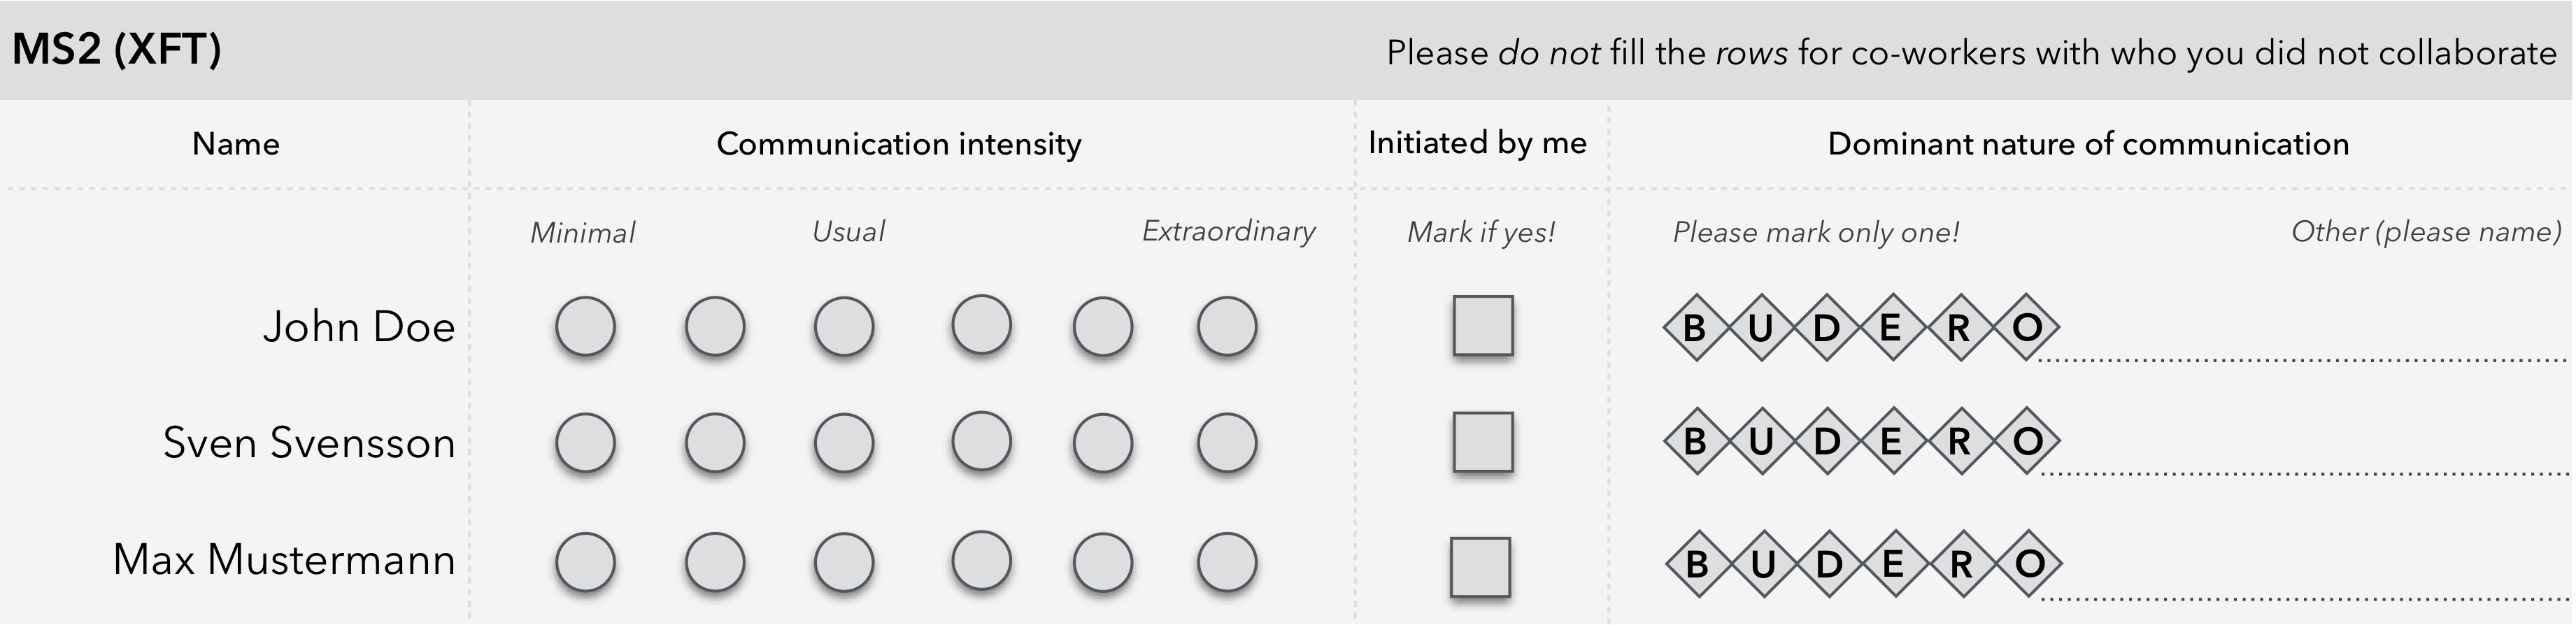
\includegraphics[width=1.0\textwidth]{figures/fake-partial-intensity.png}
  \caption{Communication intensities in daily survey}
  \label{fig:survey-intenity}
\end{figure}

The survey introduces the notion of a \emph{communication nature} (illustrated in Figure~\ref{fig:survey-natures}) aiming at capturing the main topic of communications between roles during a working day. The natures are designed to be disjoint and to capture the most prevailing reasons for communication among the survey's participants. The nature \quotes{Other (please name)} was left for participants to give a custom nature whenever none of the rest applied.
Furthermore, the classification of natures of communication are based on previous research conducted at Ericsson by \citet{nelson2013technicaldependencies} and \citet{boerjesson2013}. It has been discussed and reshaped in the course of several feedback loops to integrate insights provided by available participants of the study. This was done mainly to mitigate potential misunderstandings in phrasings so as to be able to clearly distinguish between the natures.

\begin{figure}[h!]
  \centering
  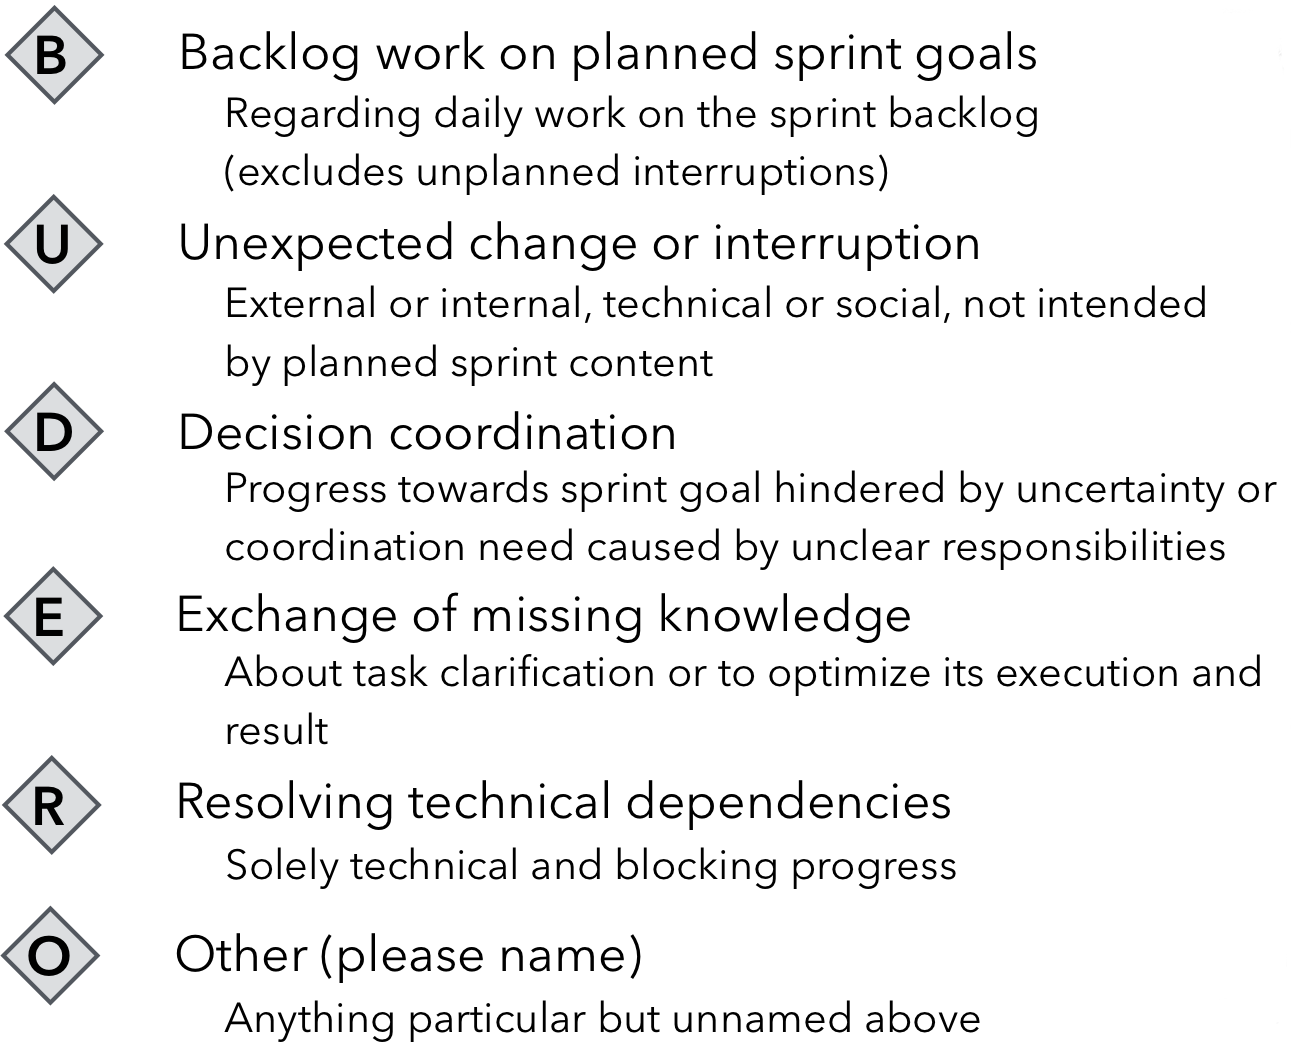
\includegraphics[width=0.60\textwidth]{figures/fake-partial-nature.png}
  \caption{Communication natures in daily survey}
  \label{fig:survey-natures}
\end{figure}

A complete example of a survey can be found in the Appendix on Figure~\ref{fig:fake-survey-1}. 

Direct administration to the respondent group allowed to control the completeness of each response and guaranteed a 100\% response rate as every participant was in personal contact with the researchers. Travelling and absence from the office caused three empty responses, resulting in 97 out of 100 possible fill-outs.

Every respondent was introduced to the survey's goals before the first day's version was handed out. The explanation included the envisioned reason and outcome of the study, data collection procedure and the outline of the main concepts of the survey, while the respondents had the possibility to ask clarifying questions.

The survey was trialled on three volunteers of which one was the participant of the actual study to obtain general feedback on apprehension of the survey and its design. It shall be noted that rooted in the survey's nature the participant was not biased by trialling. The person only gained knowledge about the survey's concepts previous to other participants.

\subsection{Interviews}

After processing the data from the surveys, semi-structured face-to-face interviews ranging from 30 to 60 minutes were conducted over a three week period. The interview guide was designed to drive the conversations with respondents, whose roles can be seen in Table \ref{table:study-participants}.
The process for this data collection method was defined in accordance with the guidelines mentioned by~\citet{runeson2012CaseStudyResearchInSE} and \citet{Myers2007ISinterview}.

\begin{table}
\begin{center}
    \begin{tabular}{ | l | l | l | }
      \hline
      \multicolumn{3}{ |c| }{\textbf{XFT-1}} \\
      \hhline{===}
      \multicolumn{1}{ |c| }{\textit{Role}} & \multicolumn{1}{ |c| }{\textit{Interview}} & \multicolumn{1}{ |c| }{\textit{Survey}} \\ \hline
      XFT Scrum Master & 1 & 1 \\ \hline
      XFT Developer & 2 & 5  \\ \hline
      XFT PG & 0 & 1 \\ \hline
      OPO & 1 & 1 \\ \hline
      Department Manager (acting Section Manager) & 1 & 1 \\ \hline
      Program Manager & 1 & 1 \\
      \hhline{===}
      \multicolumn{3}{ |c| }{\textbf{XFT-2}} \\
      \hhline{===}
      XFT Scrum Master & 1 & 1 \\ \hline
      XFT Developer & 2 & 5  \\ \hline
      XFT PG & 1 & 1 \\ \hline
      OPO & 1 & 1 \\ \hline
      Department Manager (acting Section Manager) & 1 & 1 \\ \hline
      Program Manager & 1 & 1 \\ 
      \hhline{===}
      \multicolumn{1}{ |r| }{\textit{Total}} & \textit{13} & \textit{20} \\ \hline
    \end{tabular}
\caption{Study participants}
\label{table:study-participants}
\end{center}
\end{table}

A date, time and location for each interview were discussed in advance to make sure their conduction is free of external pressures and the setting is suitable for a productive conversation. Each session begun with an introduction to the research goals and an agenda for the upcoming interview. The interviewee was then asked the permission to record the interview and was guaranteed that the response will be kept anonymous.

The questions were structured following the pyramid model, starting with more specific questions then later on transitioning towards open-ended ones~\citep{runeson2012CaseStudyResearchInSE}. A set of questions about the employee's background was asked aiming to break the ice and establish a friendly atmosphere. The main body of questions was unified by the same underlying theme derived from the research questions. Moreover, the same general guide was used for all interviewees who were not a \ac{SM} or a \ac{PgM} and was extended by a brief specific guide dependent on the interviewee's role. The separate guide was used for interviews with \acp{PgM} and \acp{SM} and is a strict subset of the general guide. The complete \nameref{app:interview-guides} can be found in the Appendix.

To finish the interview, the researchers summarized the answers allowing the interviewee to augment any part of their response if needed. The participants were asked not to discuss the interview with their colleagues until the end of the interview period to avoid a learning effect. Later on, interviewees were also provided with the transcript of their interview to correct any of the points they did not consider valid.

\subsection{Additional Data Collection Methods}

In addition to interviews and surveys, the internal documentation was also used to study the research's context. The information extracted from such sources mostly concerned issues such as organisational structure and process descriptions.
Moreover, the researchers had access to the working area of both~\acp{XFT}, which allowed for observations and possibility to ask additional questions about the working environment. The participants' observation~\citep{Lethbridge05studyingsoftware} took place at the onset of the study to integrate with the teams and establish more firm personal contact.

\section{Data Analysis}

The data analysis for both the quantitative and qualitative part of the study was performed directly after the collection. At a later stage potential relationships and correlations between data sets were pointed out to ground a deeper understanding from both data collection methods. 

\subsection{Daily Surveys}
 
The data obtained from the daily surveys was digitalized manually. To assure the correctness of the input data and minimise the possibility of human errors, both researchers processed the same response forms and cross-checked for inconsistencies after.
Data was stored in \emph{*.json}-files which were used as input for further automated calculations. Resulting data was finally transformed into \emph{*.csv}-files to generate communication heat maps with the help of the R software environment\footnote{\url{www.r-project.org}}.

Any data processing needed to generate data suitable for R was performed using a custom build software component. The software reads all survey responses from the \emph{*.json}-files and allows filtering by time, communication nature and employee's role. Filters were aimed to get a more detailed view towards specific subsets of the collected data. The functionality was tested and verified to ensure the output's correctness.
The final visualisation images were produced after the survey week using the values accumulated throughout this period.

The visualisation of the data in forms of social networks was performed using Gephi — an open source graph visualisation and manipulation software\footnote{\url{https://gephi.org/}}.

\subsection{Interviews}

The processing of the interviews data was performed using thematic analysis — a method targeted at discovering, analysing and reporting on patterns in data of qualitative nature~\citep{braun2006using}. The studied dataset consisted of the interview recordings that all together summed up to 13 data items.

%Researcher judgement is necessary to determine what a theme is. 
%determine what a "prevalence" is and be consistent about it, explain how you measure.
%literature study before the analysis - yes or no

The description of the method by \citet{braun2006using} outlines 6 phases of the process:

\begin{enumerate}
  \item \textbf{Familiarising with data.} Review of the transcriptions while keeping a focus on possibly recurring patterns.
  \item \textbf{Generating initial codes.} Categorisation of the data set to initial codes.
  \item \textbf{Searching for themes.} Initial combination of codes into themes.
  \item \textbf{Reviewing themes.} Critical reflection on completeness and correctness of themes by again investigating the coded data.
  \item \textbf{Defining and naming themes.} Further theme descriptions and reflections on its contribution to the studied issues.
  \item \textbf{Producing the report.} Selection of the most descriptive and compelling themes by aligning them to research questions.
\end{enumerate}

As a first step towards the familiarisation with the data each interview was transcribed in accordance with the intelligent verbatim format: filter words and repetitions were left out aiming to capture the information content and produce a more eloquent and concise report. Each transcript was then proof-read and summarised by both researchers. The summaries were not used within the thematic analysis and solely served the purpose of familiarising oneself with the contents of the interviews.

\section{Threats to validity}

This section discusses threats to validity of the research methodology and data collection of the study according to classification suggested by \citet{runeson}.

\subsection{Construct Validity}

Construct validity relates to the connection between operational methods and research theories investigated in the scope of the study~\citep{runeson}.

To assure a common understanding of the concepts used in data collection instruments, each survey participant went through a printed survey form together with the researchers, where the latter explained every section in detail and the former was able to ask clarifying questions. Interviewees were supplied with a study description involving goals and agendas via E-Mail before the interview and were briefly introduced this information again at the beginning of the interview session where they had the possibility to get thorough explanation on unclear parts. The evaluation apprehension threat, stemming from people being afraid of evaluation by their nature, was mitigated by guaranteeing anonymity to every study participant.

\citet{runeson} emphasise the role of the triangulation in empirical research, especially when dealing with data of qualitative nature. Using a variety of methods, data sources or theories allow for approaching the studied issue from different perspectives and providing a broader view thus increasing the precision of the study.
For this reason, the study collected data of different nature (daily surveys and interviews) from representatives of different teams and roles therefore broadening the scope of the opinions and perspectives on studied issues.
However, having a rather small sample of subjects from a single company remains a limitation to this study.

\subsection{Internal Validity}

Threats to internal validity arise from the examination of casual relations between the studied concepts~\citep{runeson}.

This study is focused on information and communication flow within the organisation and their influence on the work flow of \acp{XFT}. It is acknowledged that these factors are not the only ones affecting the productivity of the development teams but the scope of the study only investigates this perspective.

Using daily surveys to determine communication patterns is highly dependent on the respondents' answers and prone to the maturation threat. The duration of the data collection period, however, was rather short thus making motivation fluctuations and change in perceptions towards understanding of the survey's concepts rather unlikely.
To alleviate the survey's potential instrumentation flaws it was designed with the results of previous studies by~\citet{nelson2013technicaldependencies} and~\citet{boerjesson2013} and feedback of trial participants as an input. The interview instrument went through a set of feedback loops with the study's supervisors to secure understandability and comprehensiveness.

The participating \acp{XFT} may not be representative of the patterns within the whole organisation but it should be noted that the studied subjects were selected by an Agile Coach who is knowledgeable about the performance and experiences inside the organisation.

\subsection{External Validity}

External validity is concerned with generalisability of the research findings \citep{runeson}.

This study was conducted in collaboration with a single organisation hence the setting might be biased by the culture and structure of this particular organisation and consequently its interpretation of agile software development. The results therefore may not be generalisable to a full extent by the nature of a case study. The discovered problematic areas of the large-scale agile application are not necessarily valid in every context, however, a subset of the discovered challenges and proposed solutions may be transferred as an input to the investigation of another case while the discussion also aims at developing a more generalisable understanding.

\subsection{Reliability}

Reliability threats arise from the influence of the researchers on the data and its analysis~\citep{runeson}.

To enable the possibility of conducting a similar study by another researcher the steps of the data collection were documented in detail and decisions for application of research methods argued for.

The study has been performed by two researchers thus lowering the possibility of a single researcher's bias. The instruments used in the study have also been discussed with both of the study supervisors.